\scanpage{21}
- 189 - \hfill n\textsuperscript{o} 391

En effet, (§ 6, n\textsuperscript{o} 5, prop. 12), ce groupe quotient est isomorphe au sous-groupe $G_{\unsure{o|0}}$ de $A(R)$ laissant stable un système de racines simples $S(C)$ de $R$ ; il est clair que tout élément de $G_{\unsure{o|0}}$ détermine un automorphisme unique du schéma de Dynkin de $R$ relatif à $C$ ; mais inversement, un tel automorphisme se prolonge en un automorphisme unique de $R$ en vertu de la prop. 2, d'où le corollaire.

Les remarques du début et les définitions précédentes montrent que le schéma de Dynkin d'un système de racines $R$, relatif à un système de racines simples $(v_i)_{1\leq\unsure{j|i}\leq\ell}$, détermine le schéma de Coxeter du groupe de Weyl $W(R)$ de la manière suivante : les graphes sous-jacents sont les mêmes ; en outre, si $\{v_i,v_j\}$ est une arête du schéma de Dynkin, le nombre $m_{ij}$ est égal à $3$ si $f(v_i)=f(v_j)$, à $4$ si $f(v_i)/f(v_j)$ est égal à $\frac12$ ou à $2$, à $6$ si $f(v_i)/f(v_j)$ est égal à $1/3$ ou à $3$. On verra par contre ci-dessous qu'un même schéma de Coxeter peut correspondre à deux schémas de Dynkin non isomorphes, (en fait, il ne peut correspondre qu'à \uline{deux} tels schémas au plus, et cela ne se produit que pour les schémas de Coxeter de type $B_\ell$ ; pour tous les autres types, le schéma de Coxeter de $W(R)$ détermine le schéma de Dynkin de $R$ à isomorphisme près).

THEOREME 2.- \uline{Si} $R$ \uline{est un système de racines réduit irréductible}, \uline{son schéma de Dynkin est nécessairement isomorphe à l'un des suivants}, (\uline{qui sont deux à deux non isomorphes}) :

\figure{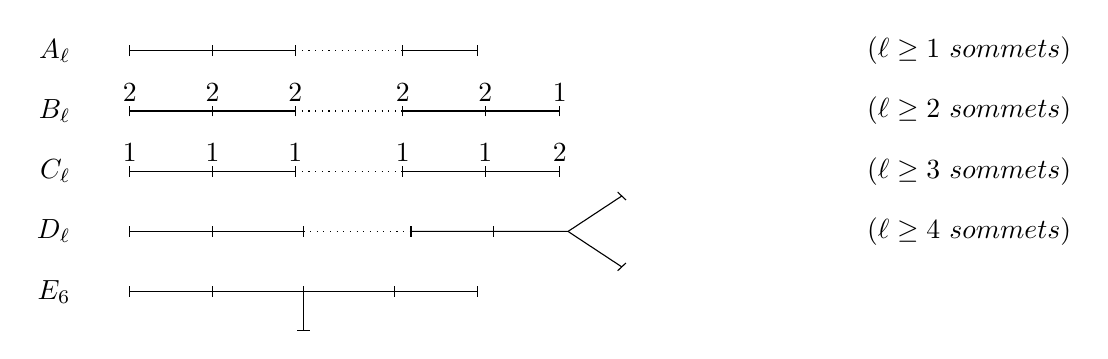
\begin{tikzpicture}[x=1.05cm,y=.9cm]
\node[left] at (-.6,0) {$A_\ell$};
\draw (0,0)--(2,0);\draw[dotted] (2,0)--(3.3,0);\draw (3.3,0)--(4.2,0);
\foreach \x in {0,1,2,3.3,4.2}{\draw (\x,-.075)--(\x,.075);}
\node[right] at (8.8,0) {$(\ell\geq1\ \uline{\text{sommets}})$};
\node[left] at (-.6,-.85) {$B_\ell$};
\draw (0,-.85)--(2,-.85);\draw[dotted] (2,-.85)--(3.3,-.85);\draw (3.3,-.85)--(5.2,-.85);
\foreach \x in {0,1,2,3.3,4.3,5.2}{\draw (\x,-.925)--(\x,-.775);}
\foreach \x in {0,1,2,3.3,4.3}{\node[above] at (\x,-.85) {$2$};}\node[above] at (5.2,-.85) {$1$};
\node[right] at (8.8,-.85) {$(\ell\geq2\ \uline{\text{sommets}})$};
\node[left] at (-.6,-1.7) {$C_\ell$};
\draw (0,-1.7)--(2,-1.7);\draw[dotted] (2,-1.7)--(3.3,-1.7);\draw (3.3,-1.7)--(5.2,-1.7);
\foreach \x in {0,1,2,3.3,4.3,5.2}{\draw (\x,-1.775)--(\x,-1.625);}
\foreach \x in {0,1,2,3.3,4.3}{\node[above] at (\x,-1.7) {$1$};}\node[above] at (5.2,-1.7) {$2$};
\node[right] at (8.8,-1.7) {$(\ell\geq3\ \uline{\text{sommets}})$};
\node[left] at (-.6,-2.55) {$D_\ell$};
\draw (0,-2.55)--(2.1,-2.55);\draw[dotted] (2.1,-2.55)--(3.4,-2.55);\draw (3.4,-2.55)--(5.3,-2.55)--(5.95,-2.05);\draw (5.3,-2.55)--(5.95,-3.05);
\foreach \x in {0,1,2.1,3.4,4.4}{\draw (\x,-2.625)--(\x,-2.475);}
\draw (5.9,-1.995)--(6,-2.105);\draw (5.9,-3.105)--(6,-2.995);
\node[right] at (8.8,-2.55) {$(\ell\geq4\ \uline{\text{sommets}})$};
\node[left] at (-.6,-3.4) {$E_6$};
\draw (0,-3.4)--(4.2,-3.4);\foreach \x in {0,1,2.1,3.2,4.2}{\draw (\x,-3.475)--(\x,-3.325);}
\draw (2.1,-3.4)--(2.1,-3.95);\draw (2.025,-3.95)--(2.175,-3.95);
\end{tikzpicture}}
\mspage{20}
